\chapter{Study of Onion Data: Collection and Analysis}


\section{System}

For now, we are working on the onion supply chain system. We have three actors in model: Farmers who are producers of onion, traders who are collectively responsible for supply of onions across country and consumers who purchase onions.

\begin{figure}[h]
\begin{center}    
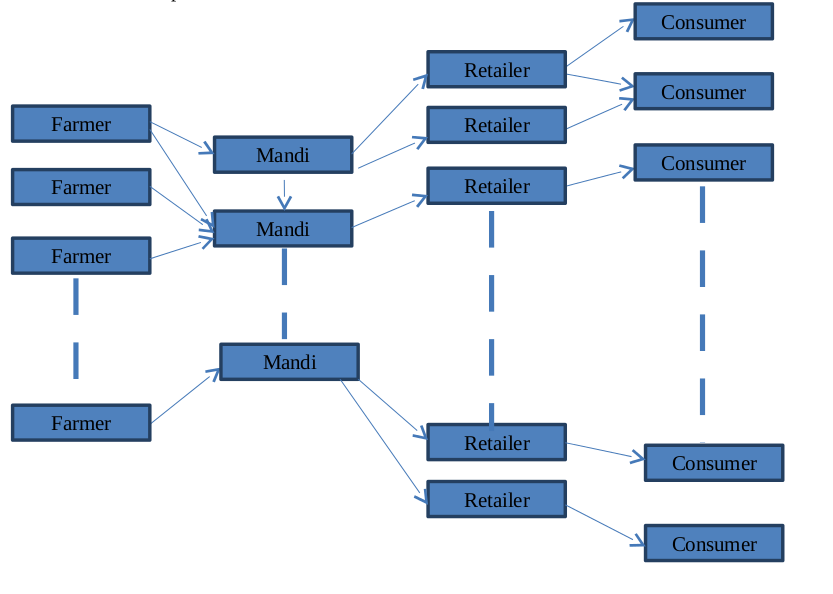
\includegraphics[scale=0.4]{3_1}
\caption{Normal Supply Chain}
\label{fig:Normal Supply Chain}
\end{center}
\end{figure}

Farmers sell their produce to traders in nearest mandi offering better price. These traders sell these commodities to traders in other mandis or to retailers. Consumers purchase commodities for consumption from one of the retail stores. This way commodity reaches consumers from farmers following a huge chain of traders and retailers.

Under APMC act, mandis were established at different places across country so that farmers can sell their produce directly in mandi and get good returns (wholesale price). There are around 1500 mandis located in different places across country which log their daily arrival of onion, minimum, maximum, modal selling price per quintal of onion data to AGMARKNET. Retailers purchase from these mandis and sell to end customers at retail price. There are around 70+ centres across country which maintains retail price of onion on Ministry of consumer affairs website.

\section{Data we have}

We have following data:

\begin{enumerate}

\item Daily wholesale price of onion for 1514 mandis
\item Daily arrival of onion information for 1514 mandis
\item Daily retail price of onion for 76 centres
\item Dates and location for hoarding reports from news articles (Total 453 news articles)
\item Longitude and latitude of mandis and centres

\end{enumerate}

Onion Data was collected from the government websites,\cite{agmarknet} for arrival and wholesale price data and \cite{retailpricecollection} (Department of Consumer Affairs) for retail price data. Crawlers were written to collect the data from these date-wise for the period of approximately 9.5 years, starting from 1st January 2006 to 6th July 2015. More data can be added simply by running crawlers again.\\
\\
Note that news articles were collected two times. First time to study what is called anomaly in the case of onion and how news source says, on what basis, that there is anomaly. We collected some set of article by manual search. We studied this to understand the characteristics of anomalies, so that we can build our system on that. These articles are studied thoroughly in this chapter in section 3.6. After that, when our system/library got ready, to match our results, we collected news articles rigorously. We have total 453 news articles regarding onion price from 1st December 2010 to 6th July 2015. First these articles were processed using Alchemy API \cite{alchemyapi} and Diffbot \cite{diffbot} to get the date, place and keywords in the article to analyse them. But we found that many of these collected articles were irrelevant, places fetched using Alchemy API was not up to the mark and date extracted from article was often wrong. Also, articles were related to onion prices. So, these APIs cannot tell us, whether article is about price hike or price dropped. Plus it was difficult for us to fetch reason of price hike from these automatic analysis
. Because of all these reasons, those articles were studied manually to find out reason stated by news articles for price hike, place mentioned in news article, number of days which are being compared to state that there is unusual price hike and any other comment if present in article. After studying each and every article manually, we found that only 267 articles are relevant to this project.


\section{Normal market behavior}

\begin{enumerate}

\item Wholesale price is inversely proportional to arrival of commodity. Higher production of crop will lead to more and more crop hitting market for sell. Hence more arrival which will result in surplus supply leading to drop in wholesale prices.

\item  Retail price is directly proportional to wholesale price. Commodities reach customers through a long chain of traders and retailers, adding value at every stage of chain. So, retail price at which customers purchase commodities are more than wholesale.

\end{enumerate}

Any divergence from these characteristics of normal market leads to suspicious price hike situations/anomalies.


\section{What are the reasons for anomaly?}

Primarily there are 3 main reasons of anomaly.

\begin{enumerate}

\item \textbf{Government Policies:} When the production is low in the country, still government allows the export of onion in large amount, or supports it by keeping low minimum price then the prices can rise up drastically.

\item \textbf{Unseasonal Rainfall:} Due to insufficient, heavy or unseasonal rainfall, onion crop may get affected and the produce is low and wholesale price may rise up. But, this reason still is validating that wholesale price is inversely proportional to arrival, it may be just prices will be little higher than what was supposed to be.

\item \textbf{Hoarding:} When traders/wholesalers store the onion and does not release the stock in the market in the expectation of the good prices in the future, it will create the artificial deficit in the market and will shoot up the onion prices in the retail market due to low arrival in the retail market. The reason people do this is to expect the higher prices in the time of low production or may be for security. For example, if it is expected that in some year the rainfall is not good, then people may predict  production to be low in the future and so they will start storing onion so that they can gain more profit. It will also create deficit in the market and price will go up.

\end{enumerate}

So our study will focus on detection of anomalies in data and if possible comment on the possible reason for the anomaly.

\section{Mapping of wholesale price to retail price}

Voronoi Diagram is used to map every mandi to nearest possible centre. The centres with retail data were considered fixed points and country was divided into 76 regions. All the mandis falling in that region are mapped to the respective centre.


\begin{figure}[h]
\begin{center}    
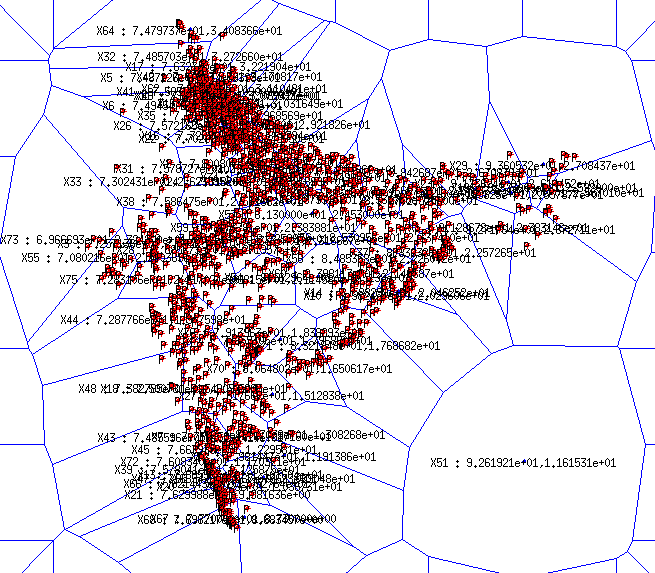
\includegraphics[scale=0.7]{3_2}
\caption{Voronoi Diagram}
\label{fig:Voronoi Diagram}
\end{center}
\end{figure}


After all the mandis are mapped to their nearest centre, wholesale and arrival at every centre is computed. Wholesale price at centre is average of modal price of all mandis in its region and arrival was computed as the sum of the arrival at the mandis in its region. While calculating the wholesale price, the distance between centre and the mandi was not considered.




\section{How to Define Anomaly?}

To answer this question, we went through the series of the news articles when the hoarding is in the news. Then looking over those articles, we try to see that why they are reporting in news, what happened so that these news articles are calling it a case of hoarding.

\subsection{Summary Of News Articles}


First such incident was reported in the 1998. The article \cite{Redif57:online} dated on 21st September 1999 states as follows:

\textit{"Onions were retailed at Rs 6 a kilo two weeks back. Today, the price was almost 100 per cent up, hovering in the Rs 10-12 band in different parts of the country."}

So this article is comparing the retail price of today with the price before 2 weeks. The rise upto 100\% is what has come to notice. Also article says that,

\textit{"There is talk in the market that the government is likely to lift the ban on onion exports. Apparently, some traders are resorting to hoarding in anticipation of demand from markets abroad."}

As stated previously also, government policy also plays a major role in this. After that Onion was in news in 2010. NDTV \cite{Whyo17:online}, TOI \cite{Theg44:online} and many more reported the incident. In 2010, unseasonal rainfall and the government policy on export price were also the reason for hike in the price. The report dated Dec 23, 2010, TOI states the follows (in Delhi):

\textit{"On Tuesday alone, wholesale traders in Delhi bought onions at about Rs 34 per kg while it was sold in retail at Rs 80 per kg. That's a margin of Rs 46 per kg or 135\%!" }

Here, they have compared the difference between the wholesale price and the retail price. The margin of 135\% is reported. When we looked into data we have, we got the following results for Dec, 2010. (See figures \ref{fig:DelhiDec2010} and \ref{fig:DelhiDec2010Relativedifference})

\begin{figure}[h]
\begin{center}    
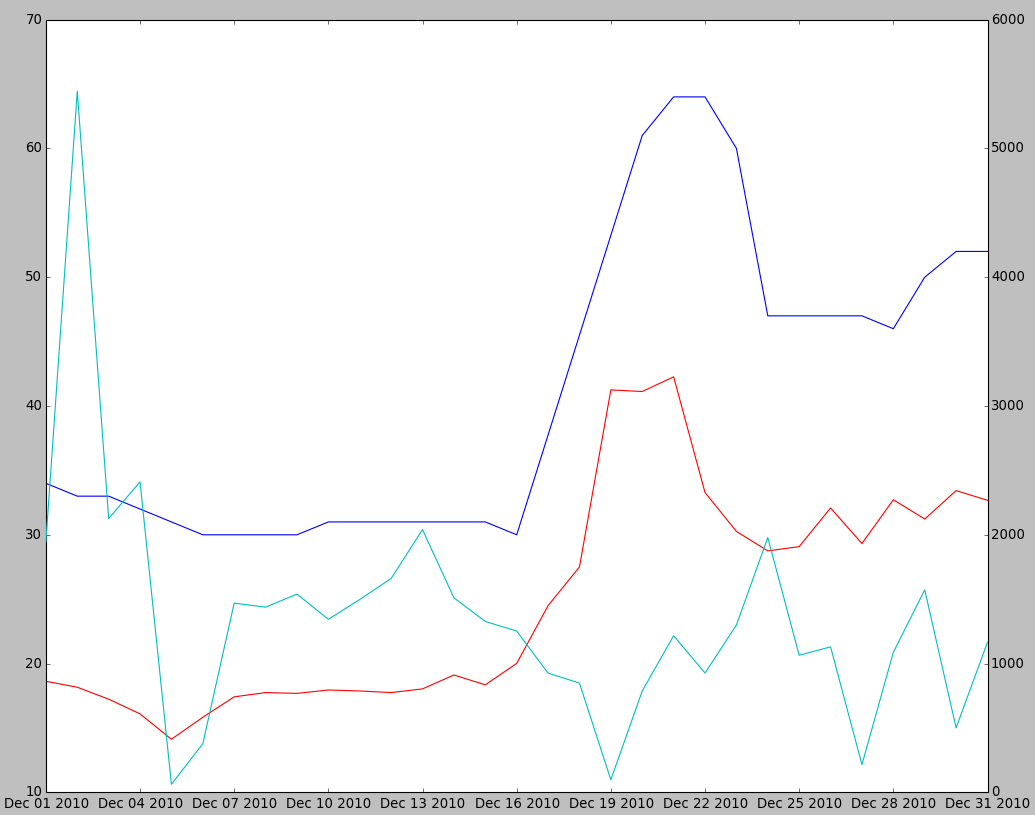
\includegraphics[scale=0.3]{2010_dec_delhi}
\caption{Delhi, Dec 2010. (Blue - Retail price, Red - Wholesale Price, Cyan - Arrival)}
\label{fig:DelhiDec2010}
\end{center}
\end{figure}

\begin{figure}[h]
\begin{center}    
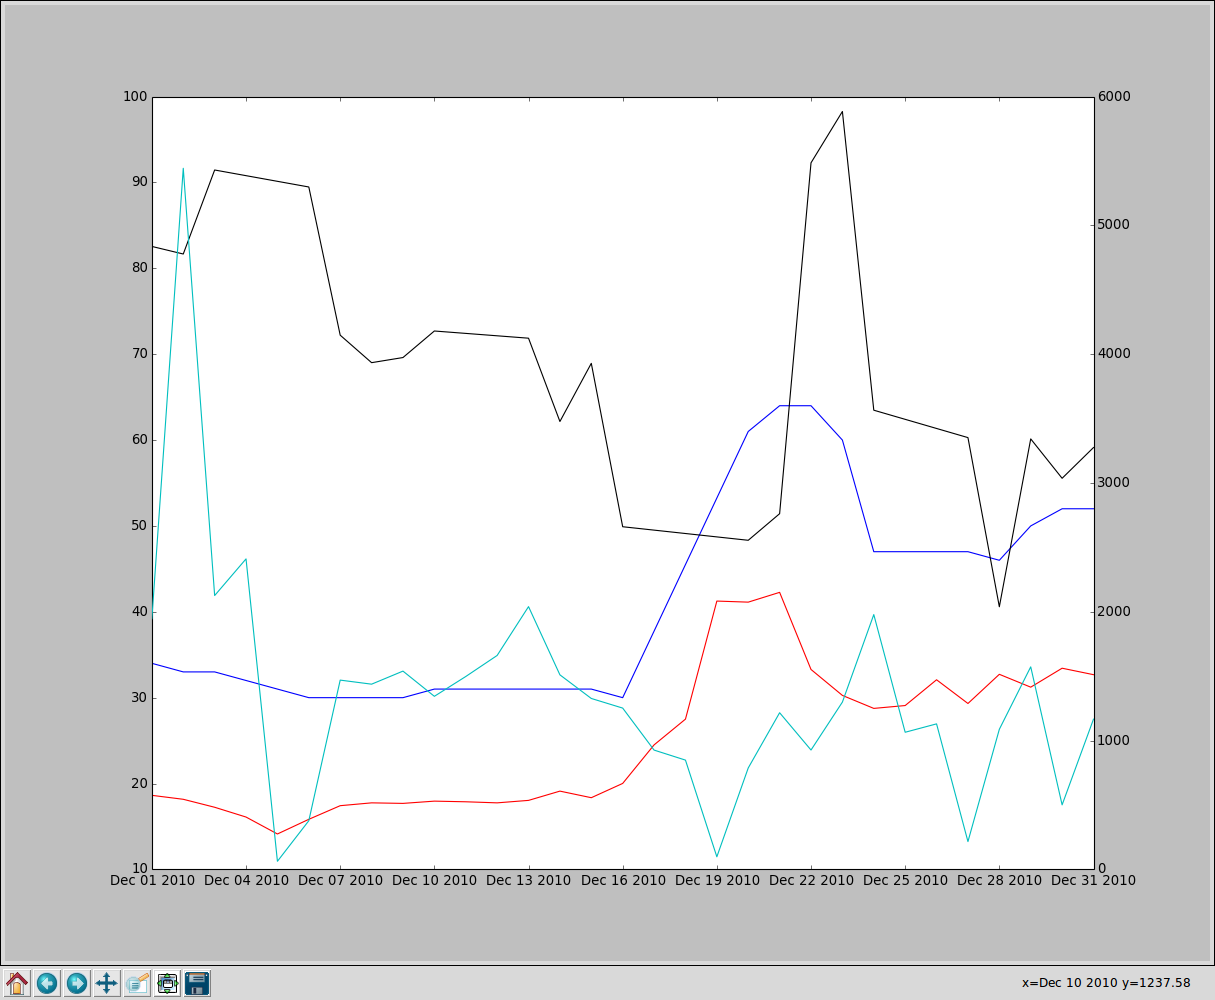
\includegraphics[scale=0.3]{2010_dec_delhi_with_relative_diff}
\caption{Delhi, Dec 2010. (Blue - Retail price, Red - Wholesale Price, Cyan - Arrival,Black - Relative difference \%)}
\label{fig:DelhiDec2010Relativedifference}
\end{center}
\end{figure}

So, as per our data, the maximum price difference observed was of \~ 100\% . Note that the retail prices we have is the minimum price observed in the market.

NDTV on Dec 22, 2010 reported the following (NASIK):

\textit{"The average purchase rate of a trader here is about Rs. 3,000, but they go to the cities and claim it's nearly Rs. 8,000 and that's how the rates go up. It's all the fault of the traders. They loot the people," said Sangdeorao Holkar, Director, National Agricultural Cooperative Marketing Federation of India.}

Here also, as we see they have mentioned price difference between retail and wholesale in the market. It is approximately \~166\%.

Report also adds the following:

\textit{“The government, on a back foot, banned exports last evening. In less than 24 hours, prices in Lasalgaon crashed by 25 per cent.}\\
\begin{center}
\textit{Navi Mumbai: Wholesale price } \\
\textit{Tuesday: Rs. 60 per kg }\\
\textit{Wednesday: Rs. 45 per kg }
\end{center}
\textit{And this is finally what the consumer in Mumbai is paying:}
\begin{center}
\textit{Mumbai: Retail price}\\
\textit{Tuesday: Rs. 60 to Rs. 70 per kg}\\
\textit{Wednesday: Rs. 60 to Rs. 70 per kg” }
\end{center}
So as we can see, there is significant drop in the wholesale price, but no drop in the retail price, so that has been reported. Also difference in the hike in retail price, from 40 to 60 was reported in on week. What our data says:

\begin{figure}[h]
\begin{center}    
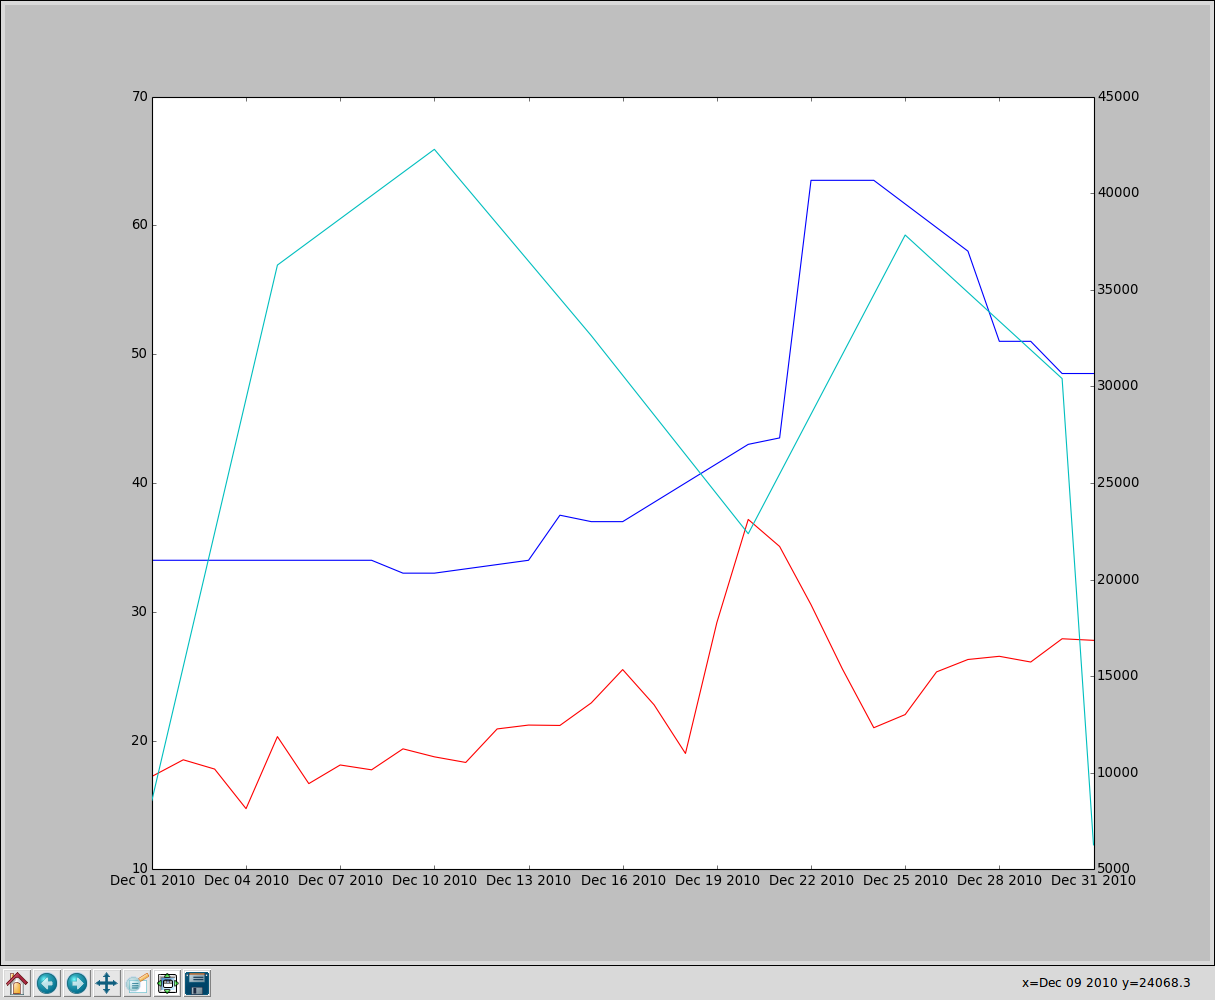
\includegraphics[scale=0.3]{2010_dec_maha}
\caption{Maharashtra, Dec 2010. (Blue - Retail price, Red - Wholesale Price, Cyan - Arrival)}
\label{fig:MaharashtraDec2010}
\end{center}
\end{figure}

\begin{figure}[h]
\begin{center}    
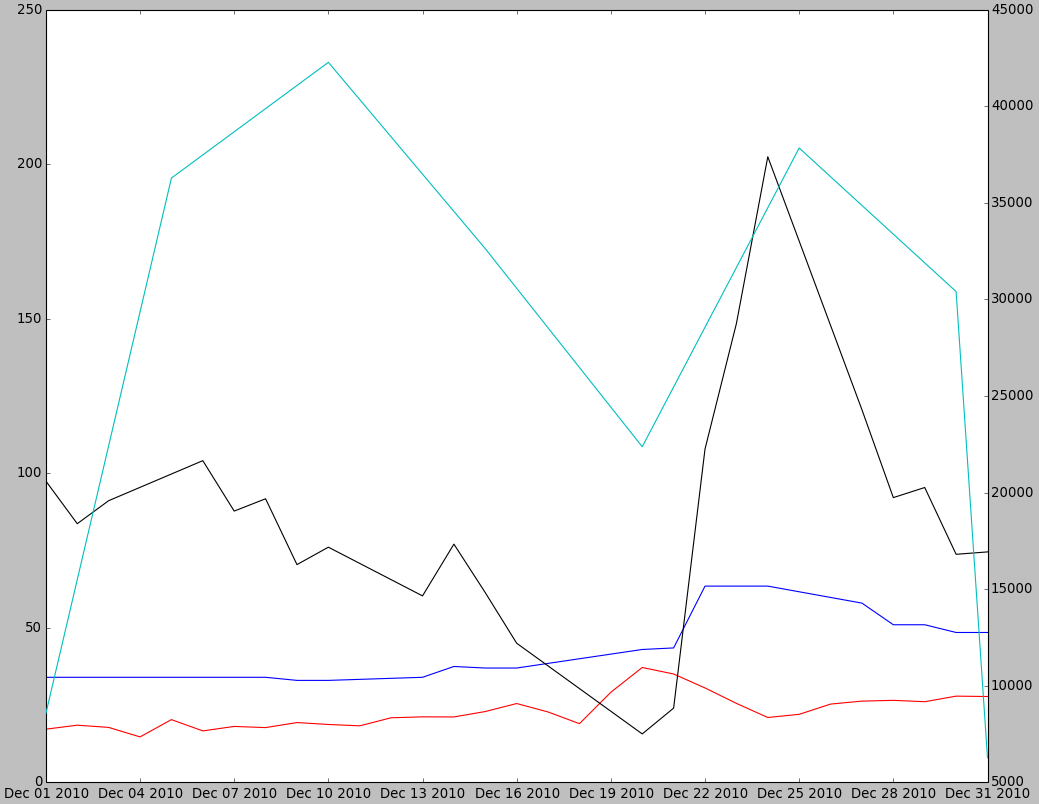
\includegraphics[scale=0.3]{2010_dec_maha_relative}
\caption{Maharashtra Dec 2010. (Blue - Retail price, Red - Wholesale Price, Cyan - Arrival, Black - Relative difference \%)}
\label{fig:MaharashtraDec2010Relativedifference}
\end{center}
\end{figure}

\begin{figure}[h]
\begin{center}    
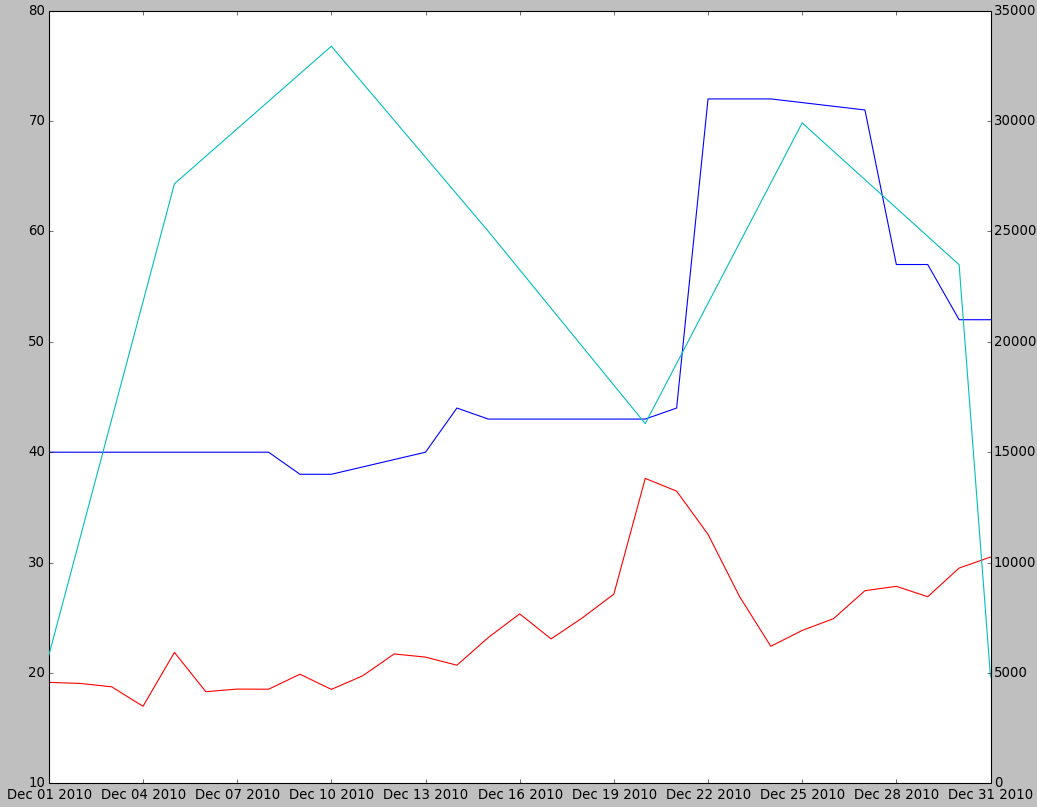
\includegraphics[scale=0.3]{2010_dec_mumbai}
\caption{Mumbai , Dec 2010. (Blue - Retail price, Red - Wholesale Price, Cyan - Arrival)}
\label{fig:MumbaiDec2010}
\end{center}
\end{figure}

\begin{figure}[h]
\begin{center}    
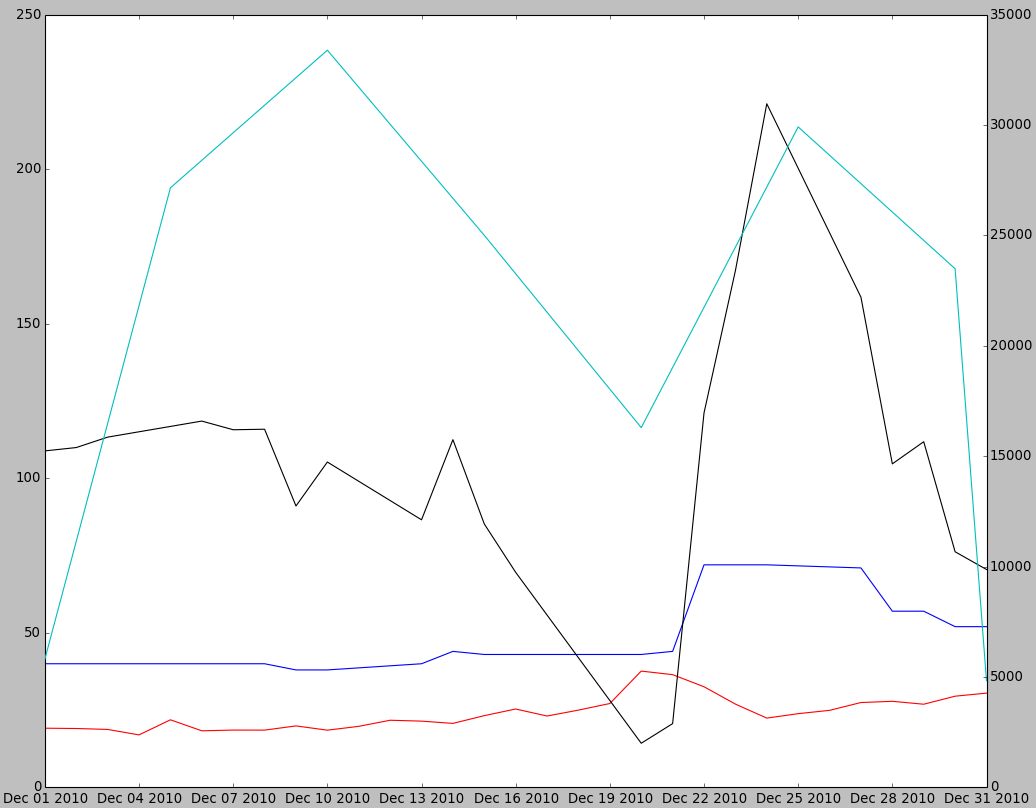
\includegraphics[scale=0.3]{2010_dec_mumbai_relative}
\caption{Mumbai, Dec 2010. (Blue - Retail price, Red - Wholesale Price, Cyan - Arrival Black - Relative difference \%)}
\label{fig:MumbaiDec2010Relativedifference}
\end{center}
\end{figure}

As we can see from the Figures \ref{fig:MaharashtraDec2010}, \ref{fig:MaharashtraDec2010Relativedifference}, \ref{fig:MumbaiDec2010} and \ref{fig:MumbaiDec2010Relativedifference}, the difference between retail and wholesale went as much high as 200\% in both overall Maharashtra as well as in the Mumbai. Also, as per report \cite{Theg88:online}, this trend was also continued in the next month, i.e. January 2011, which can be seen in the following graph. (See figures \ref{fig:MumbaiJan2011} and \ref{fig:MumbaiJan2011Relativediff}) \\

\begin{figure}[h]
\begin{center}    
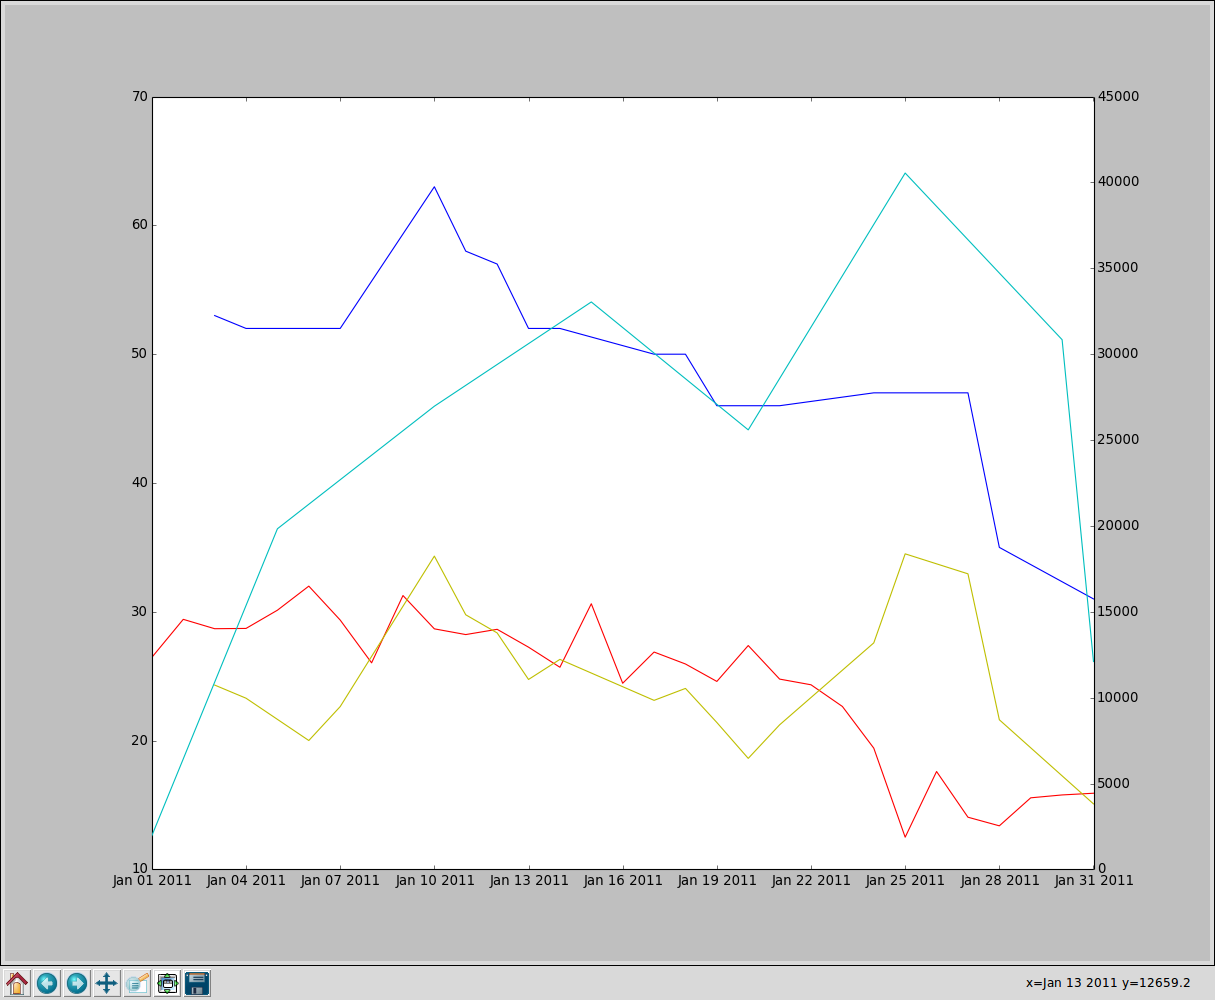
\includegraphics[scale=0.3]{2011_jan_mumbai}
\caption{Mumbai , Jan 2011. (Blue - Retail price, Red - Wholesale Price, Cyan - Arrival)}
\label{fig:MumbaiJan2011}
\end{center}
\end{figure}

\begin{figure}[h]
\begin{center}    
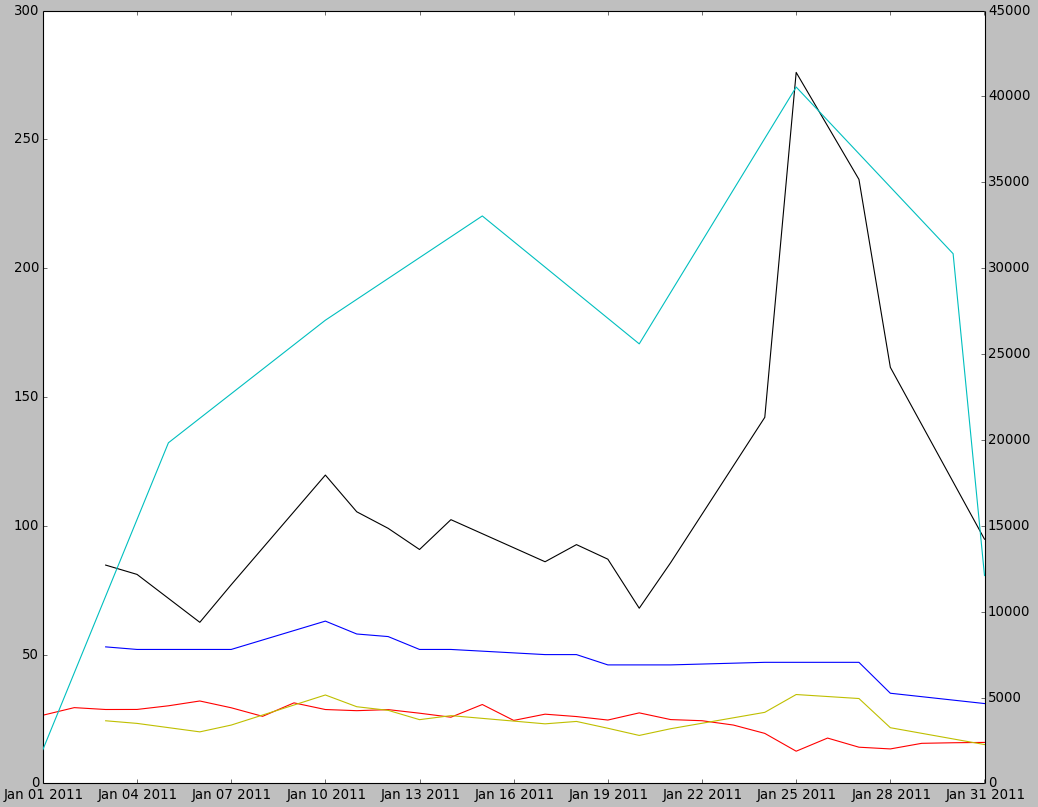
\includegraphics[scale=0.3]{2011_jan_mumbai_relative_diff}
\caption{Mumbai, Jan 2011. (Blue - Retail price, Red - Wholesale Price, Cyan - Arrival Black - Relative difference \%)}
\label{fig:MumbaiJan2011Relativediff}
\end{center}
\end{figure}

Next hoarding news was reported in the last week July 2013. As per the Business Standard Report \cite{Flyin19:online},\\

\textit{"Onion prices in Nashik, Pune and Ahmednagar have increased to Rs 2,400 a quintal as on July 21, compared to Rs 1,500-1,800 a quintal during the corresponding period of last year. Arrival of onions in Nashik, which contributes 35-40 per cent to the state production, has been 83,000 quintals compared with 82,000 quintals last year"}\\

Also, In the month of August, September and October of 2013, the price rise of the Onion in various parts of countries like Banglore (\cite{Onion55:online}), New Delhi (\cite{Hoard62:online},\cite{Onion85:online},\cite{Noon17:online}) and Gandhinagar ([\cite{Govt81:online}) was in the news. Reports of Banglore and New Delhi has just reported the hike in the retail price. DNA report on Gandhinagar says,\\

\textit{"Retail onion prices in the city have increased from around Rs. 40 per kg, a month ago, to Rs. 70/kg on Saturday. In the wholesale market, onion prices have increased around Rs. 35 per kg till last week to Rs. 45 per kg on Saturday. The wholesale price is Rs. 40 to 45 per kg. Ideally, in the retail market the price should not be more than Rs. 60 per kg"}

Let's look at the data we have. As from the figures \ref{fig:MumbaiJuly2012} and \ref{fig:MumbaiJuly2013}, the wholesale rates around the mandis present around the Mumbai in the month of July, 2012 was about Rs. 5/Kg, but during the same time period in the 2013, the wholesale prices went from Rs. 15/Kg to Rs. 25/Kg. Although, there was decrement in the arrival by 7\% as compared to July 2012, but the rise in the wholesale price is very much high.\\

\begin{figure}[h]
\begin{center}    
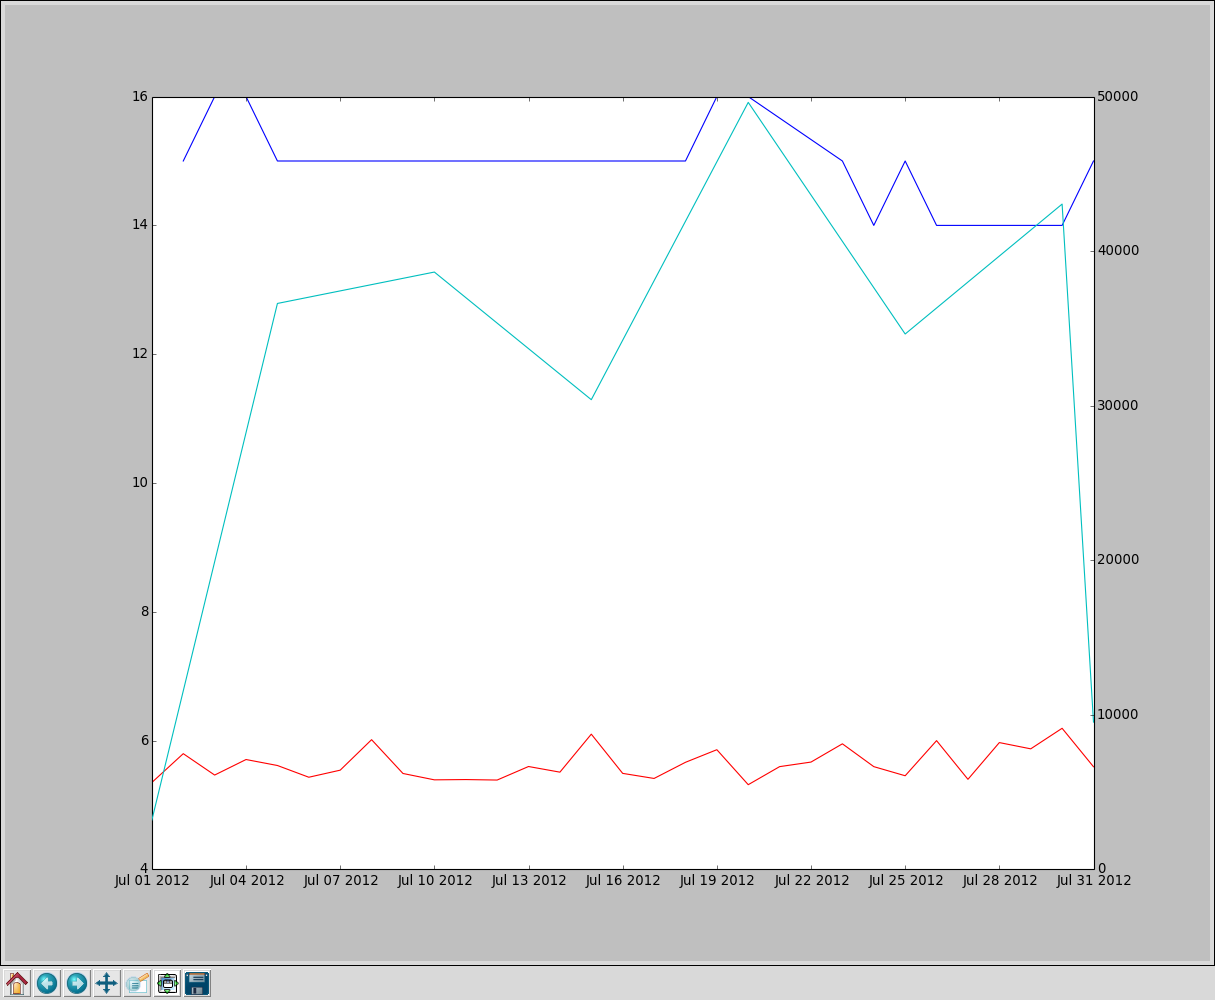
\includegraphics[scale=0.3]{2012_jul_mumbai}
\caption{Mumbai , July 2012. (Blue - Retail price, Red - Wholesale Price, Cyan - Arrival)}
\label{fig:MumbaiJuly2012}
\end{center}
\end{figure}

\begin{figure}[h]
\begin{center}    
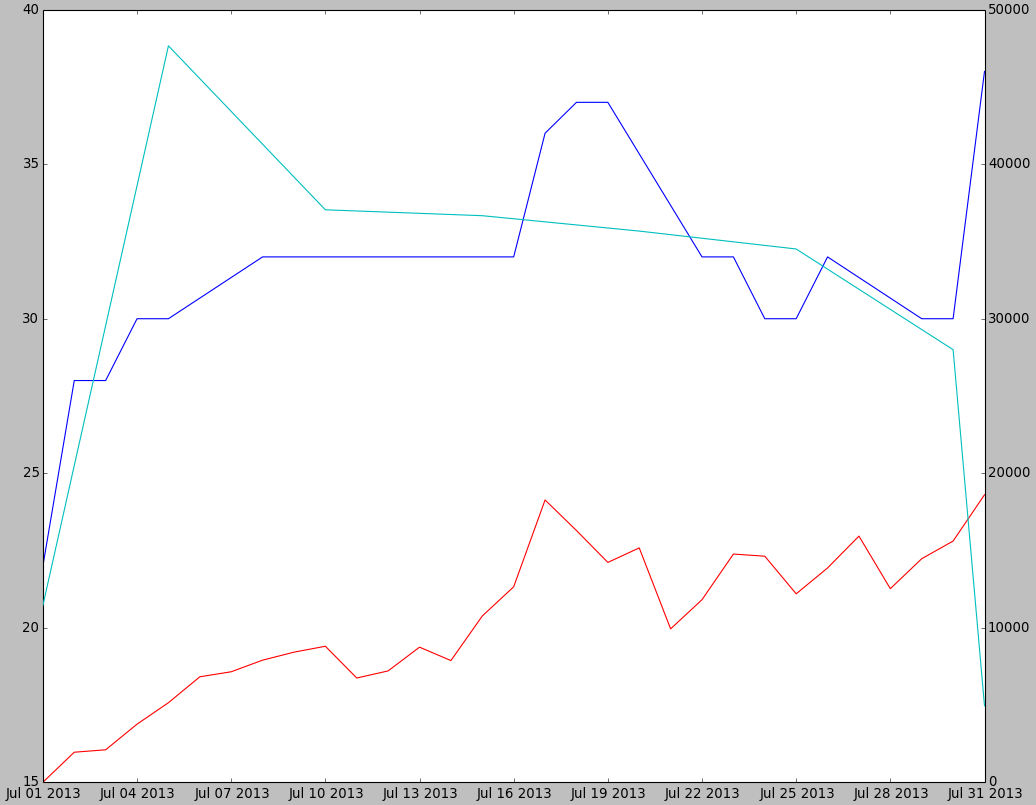
\includegraphics[scale=0.3]{2013_july_mumbai}
\caption{Mumbai , July 2013. (Blue - Retail price, Red - Wholesale Price, Cyan - Arrival)}
\label{fig:MumbaiJuly2013}
\end{center}
\end{figure}


Figures \ref{fig:AhmedabadAug2013} and \ref{fig:RajkotAug2013}, states the scenario of Gujarat. There also the wholesale as well as the retail prices became suddenly almost double in the month of August 2013. \\

\begin{figure}[h]
\begin{center}    
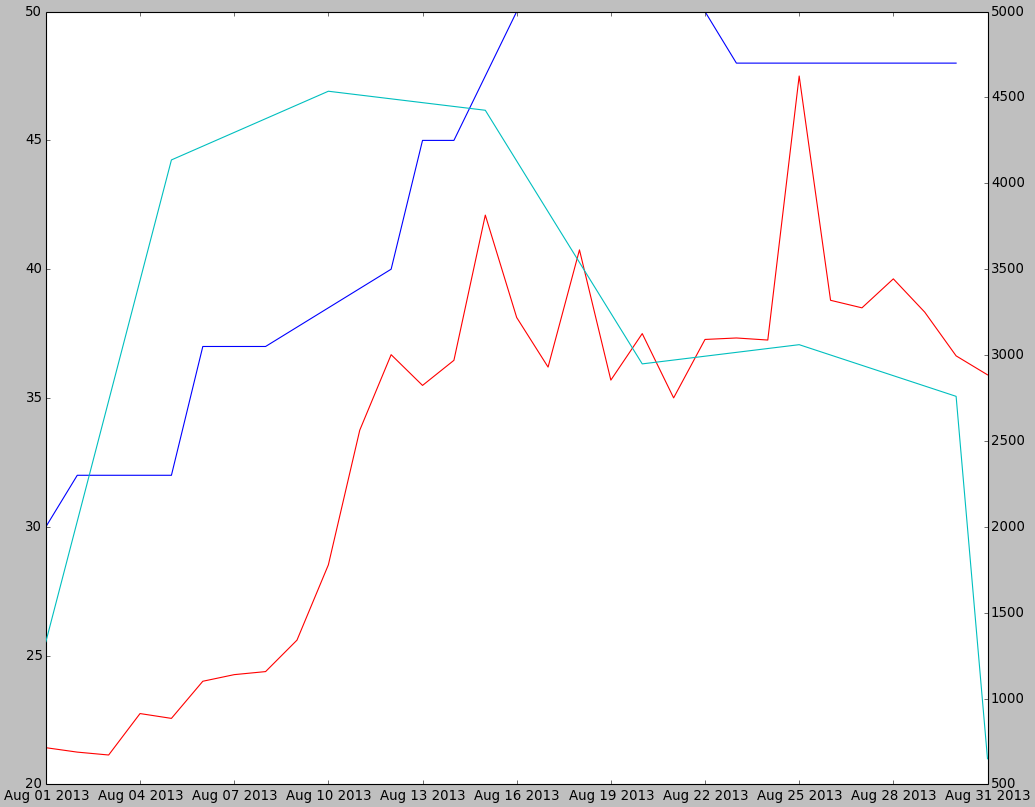
\includegraphics[scale=0.3]{2013_aug_ahmdb}
\caption{Ahmedabad , Aug 2013. (Blue - Retail price, Red - Wholesale Price, Cyan - Arrival)}
\label{fig:AhmedabadAug2013}
\end{center}
\end{figure}

\begin{figure}[h]
\begin{center}    
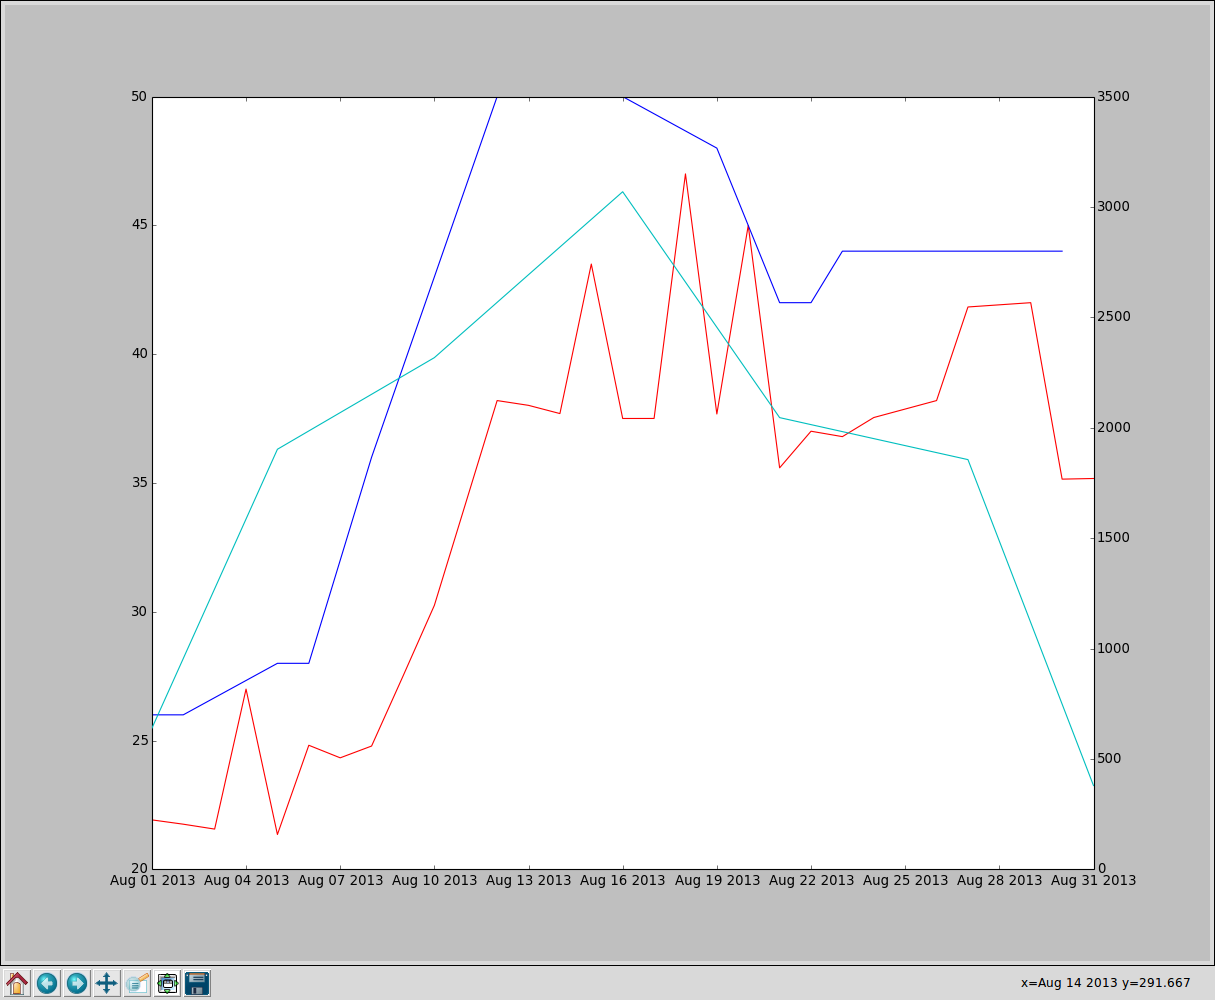
\includegraphics[scale=0.3]{2013_aug_rajkot}
\caption{Rajkot , Aug 2013. (Blue - Retail price, Red - Wholesale Price, Cyan - Arrival)}
\label{fig:RajkotAug2013}
\end{center}
\end{figure}

Also, in year 2014, price hike of Onions was in the news. There were reports from Mumbai \cite{Onion68:online}, Kerala \cite{Keral99:online} and Hydrabad \cite{Rains78:online} which stated the hike in the prices of the onion. Let's look at the graph of the Mumbai for the year of 2014. As we can see from the graph (Figure \ref{fig:Mumbai2014}) that for the period of July to October the wholesale price were decreasing, but still that was not reflected in the retail price and instead of decreasing, the retail price kept on increasing.\\


\begin{figure}[h]
\begin{center}    
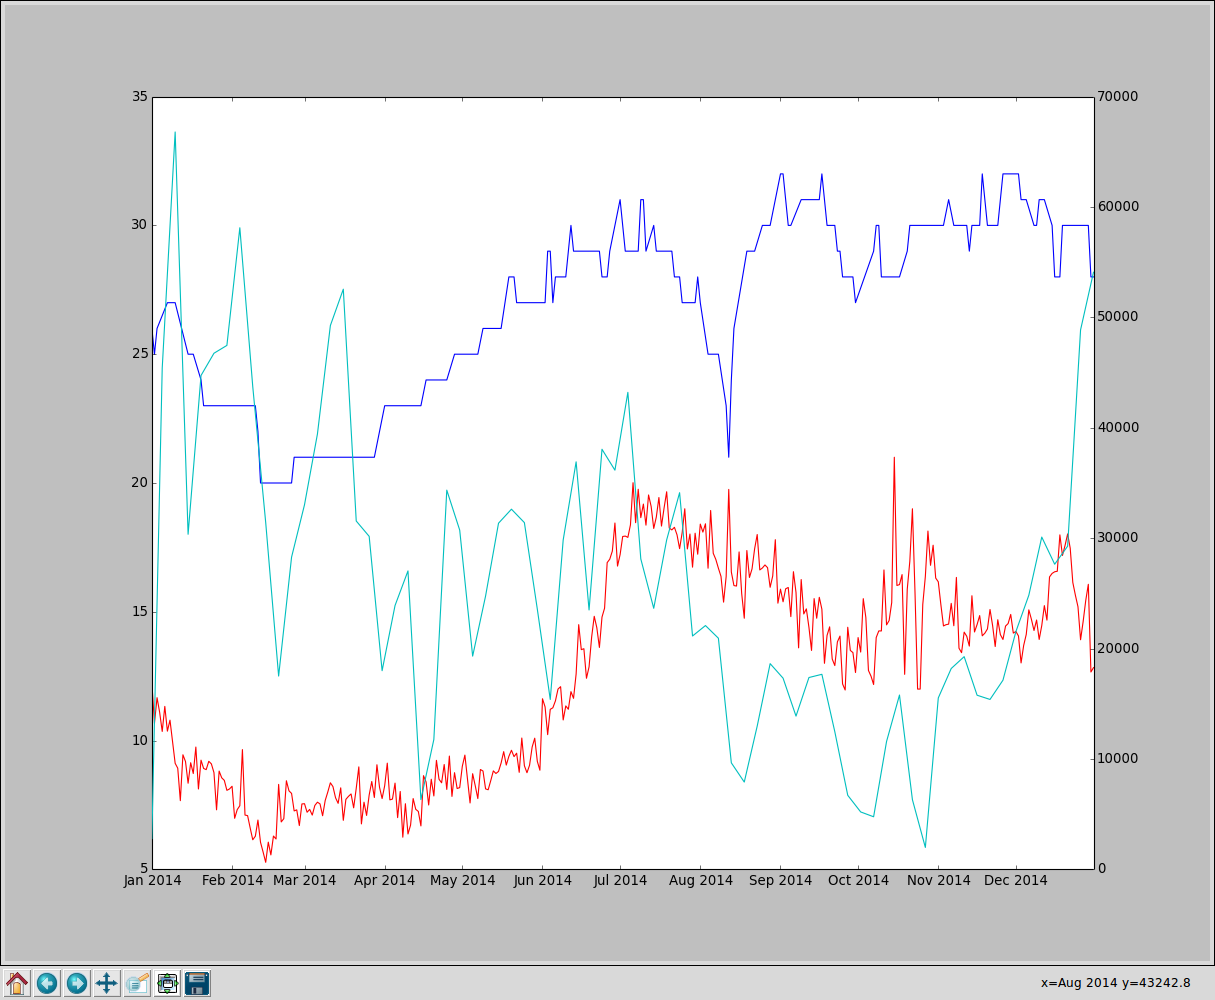
\includegraphics[scale=0.3]{2014_mumbai}
\caption{Mumbai , 2014. (Blue - Retail price, Red - Wholesale Price, Cyan - Arrival)}
\label{fig:Mumbai2014}
\end{center}
\end{figure}

\section{Characteristics of anomaly}

Hoarding of commodities in excess, results in anomaly. We segregated news articles on hoarding of onion and tried to spot some characteristics of data for anomalies.

So, major characteristics of hoarding spotted in newspapers are following:

\begin{enumerate}
\item Huge difference in wholesale and retail prices
\item Sudden rise in wholesale or retail price
\item Rise in wholesale prices when arrival is enough/high
\end{enumerate}

We can also generalize anomaly cases as shown in table \ref{table:1} and \ref{table:2}. The estimated arrival, wholesale and retail price data is labelled up, down and constant based on if it exceeds actual data value. Red flags are raised based on the following tables if the condition falls under the category marked with {\color{red}A}’s.


\begin{table}
\centering
\begin{tabular}{ | c | c | c | c |}  
  \hline
  \textbf{R$\backslash$W} & \textbf{$\uparrow$} & \textbf{$\leftrightarrow$}  & \textbf{$\downarrow$} \\ \hline
  \textbf{$\uparrow$} & - & {\color{red}A} & {\color{red}A} \\ \hline
  \textbf{$\leftrightarrow$} & - & - & {\color{red}A} \\ \hline
  \textbf{$\downarrow$} & - & - & - \\ \hline
\end{tabular}
\caption{Anomaly Scenarios - 1}
\label{table:1}
\end{table}

\begin{table}
\centering
\begin{tabular}{ | c | c | c | c |}  
  \hline
  \textbf{W$\backslash$A} & \textbf{$\uparrow$} & \textbf{$\leftrightarrow$}  & \textbf{$\downarrow$} \\ \hline
  \textbf{$\uparrow$} & {\color{red}A} & {\color{red}A} & - \\ \hline
  \textbf{$\leftrightarrow$} & {\color{red}A} & - & - \\ \hline
  \textbf{$\downarrow$} & - & - & - \\ \hline
\end{tabular}
\caption{Anomaly Scenarios - 2}
\label{table:2}
\end{table}

\section{Hypothesis}

So from the above analysis of all news reports, we conclude four hypothesis.

Wholesale price is inversely proportional to arrival in the market and we assume it is the only factor on which wholesale price is dependent. We also noticed in our literature review that most of the farmers don't hoard in India. So, from this relation, we have the following hypothesis:

\textbf{\textit{H1. If there is increase in arrival pattern, there should be decrease in the wholesale price and if there is decrease in arrival pattern, there should be increase in the wholesale price considering a lag factor of 15 days.}}

Retailers purchase onions from the wholesale markets, mandis, etc. So, rate at retail level should be directly proportional to wholesale price in that region. We assume here that demand remains constant and there is no supply shock created because of excessive export of onion So from here we get the following hypothesis.

\textbf{\textit{H2. If there is increase in the wholesale price of onion, then there will be corresponding increase in the retail price and vice-versa assuming demand remains constant and there is no supply shock created because of excessive export of onion.}}

Similarly, we can state that if there is no change in the arrival for some period, then wholesale may remain same and if wholesale price remains same for some period than retail price may remain same. So from that we get following two hypothesis:

\textbf{\textit{H3. The deviation between arrival - wholesale and wholesale- retail should not vary much compared to values for same time in past years.}}

Also, one should make a note of that, even in H1 and H2, when wholesale price or retail is increasing, then it should be in considerable amount. It should not be like, there is marginal increase in wholesale price and retail price is boosting up or there is little decrement in arrival and wholesale price goes up by unacceptable level.

Also, we assume that mandis in the same region will behave in similar manner, because production and effect of other factors will be same in one region. So, based on that we have following hypothesis:

\textbf{\textit{H4. Mandis in the same region should follow the same relationship between arrival and wholesale price, as that of, taken whole region altogether.}
\center{OR} \\
\textit{Retail prices across various centres should follow same relationship among themselves taken effect of them combinely.} }

So we have created a library which takes all these series as an input and try to detect possibilities of above stated anomalies or highlight all the important unusual behavior of parameters seen in the input series.


